\begin{appendices}
  \chapter{Appendix}
  \section{Relative Water Content - Devils Ivy}
  \begin{table}[htb]
    \centering
    \begin{tabular}{lllll}
      \toprule
      \textbf{Leaf} & \textbf{TFW} & \textbf{TW} & \textbf{DW} & \textbf{RWC} \\
      \midrule
        \texttt{11} & 2.7931 & 2.8335 & 0.2472 & 98.4379 \\
        \texttt{12} & 2.0883 & 2.1184 & 0.1876 & 98.4411 \\
        \texttt{21} & 1.7804 & 1.8051 & 0.1376 & 98.5187 \\
        \texttt{22} & 1.7655 & 1.8022 & 0.1404 & 97.7916 \\
        \texttt{31} & 2.1874 & 2.2359 & 0.1656 & 97.6573 \\
        \texttt{32} & 2.2511 & 2.3108 & 0.1687 & 97.2130 \\
        %
        \texttt{1\_1} & 2.7931 & 2.8335 & 0.2472 & 98.4379 \\
        \texttt{1\_2} & 2.0883 & 2.1184 & 0.1876 & 98.4411 \\
        \texttt{2\_1} & 1.7804 & 1.8051 & 0.1376 & 98.5187 \\
        \texttt{2\_2} & 1.7655 & 1.8022 & 0.1404 & 97.7916 \\
        \texttt{3\_1} & 2.1874 & 2.2359 & 0.1656 & 97.6573 \\
        \texttt{3\_2} & 2.2511 & 2.3108 & 0.1687 & 97.2130 \\
        %
        \texttt{11} & 2.7931 & 2.8335 & 0.2472 & 98.4379 \\
        \texttt{12} & 2.0883 & 2.1184 & 0.1876 & 98.4411 \\
        \texttt{21} & 1.7804 & 1.8051 & 0.1376 & 98.5187 \\
        \texttt{22} & 1.7655 & 1.8022 & 0.1404 & 97.7916 \\
        \texttt{31} & 2.1874 & 2.2359 & 0.1656 & 97.6573 \\
        \texttt{32} & 2.2511 & 2.3108 & 0.1687 & 97.2130 \\
        %
        \texttt{11} & 2.7931 & 2.8335 & 0.2472 & 98.4379 \\
        \texttt{12} & 2.0883 & 2.1184 & 0.1876 & 98.4411 \\
        \texttt{21} & 1.7804 & 1.8051 & 0.1376 & 98.5187 \\
        \texttt{22} & 1.7655 & 1.8022 & 0.1404 & 97.7916 \\
        \texttt{31} & 2.1874 & 2.2359 & 0.1656 & 97.6573 \\
        \texttt{32} & 2.2511 & 2.3108 & 0.1687 & 97.2130 \\
        %
        \texttt{11} & 2.7931 & 2.8335 & 0.2472 & 98.4379 \\
        \texttt{12} & 2.0883 & 2.1184 & 0.1876 & 98.4411 \\
        \texttt{21} & 1.7804 & 1.8051 & 0.1376 & 98.5187 \\
        \texttt{22} & 1.7655 & 1.8022 & 0.1404 & 97.7916 \\
        \texttt{31} & 2.1874 & 2.2359 & 0.1656 & 97.6573 \\
        \texttt{32} & 2.2511 & 2.3108 & 0.1687 & 97.2130 \\
        %
        \texttt{11} & 2.7931 & 2.8335 & 0.2472 & 98.4379 \\
        \texttt{12} & 2.0883 & 2.1184 & 0.1876 & 98.4411 \\
        \texttt{21} & 1.7804 & 1.8051 & 0.1376 & 98.5187 \\
        \texttt{22} & 1.7655 & 1.8022 & 0.1404 & 97.7916 \\
        \texttt{31} & 2.1874 & 2.2359 & 0.1656 & 97.6573 \\
        \texttt{32} & 2.2511 & 2.3108 & 0.1687 & 97.2130 \\
        %
        \texttt{11} & 2.7931 & 2.8335 & 0.2472 & 98.4379 \\
        \texttt{12} & 2.0883 & 2.1184 & 0.1876 & 98.4411 \\
        \texttt{21} & 1.7804 & 1.8051 & 0.1376 & 98.5187 \\
        \texttt{22} & 1.7655 & 1.8022 & 0.1404 & 97.7916 \\
        \texttt{31} & 2.1874 & 2.2359 & 0.1656 & 97.6573 \\
        \texttt{32} & 2.2511 & 2.3108 & 0.1687 & 97.2130 \\
      \bottomrule
    \end{tabular}
    \caption{%
      Measurements for RWC Experiment
    }
    \label{tab:Packages}
  \end{table}
  \section{Additional GLCM Results - Red Oak}
  %\subsection{Specular Results - All Species}
  \begin{sidewaysfigure}
      \begin{center}
          \makebox[\textwidth]{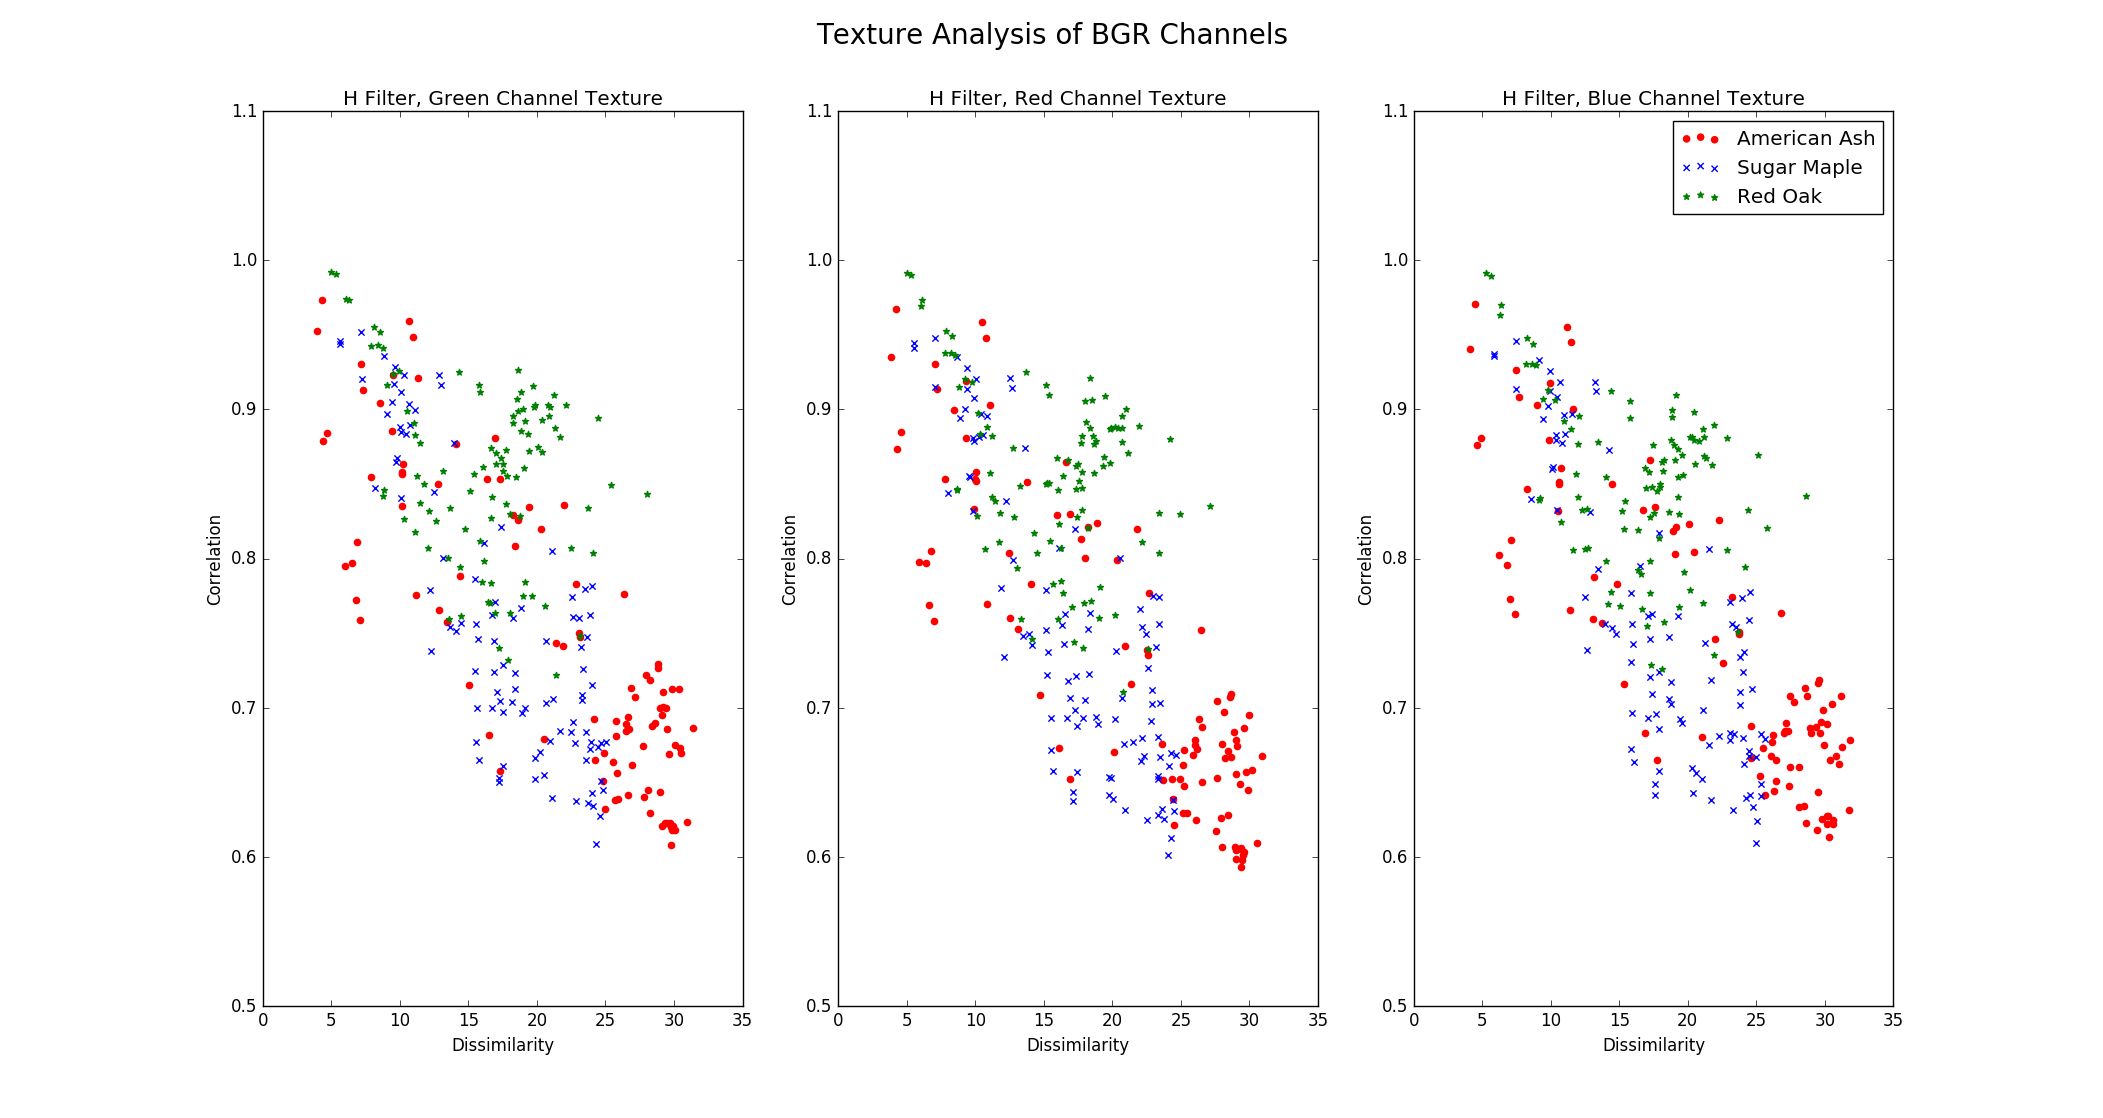
\includegraphics[scale=0.5]{/Sources/Appendix/GLCM-all-specles-H-specular.png}}
      \end{center}
      \caption{H filter GLCM Specular - All Species}
      \label{fig:polarization}
  \end{sidewaysfigure}
  \begin{sidewaysfigure}
      \begin{center}
          \makebox[\textwidth]{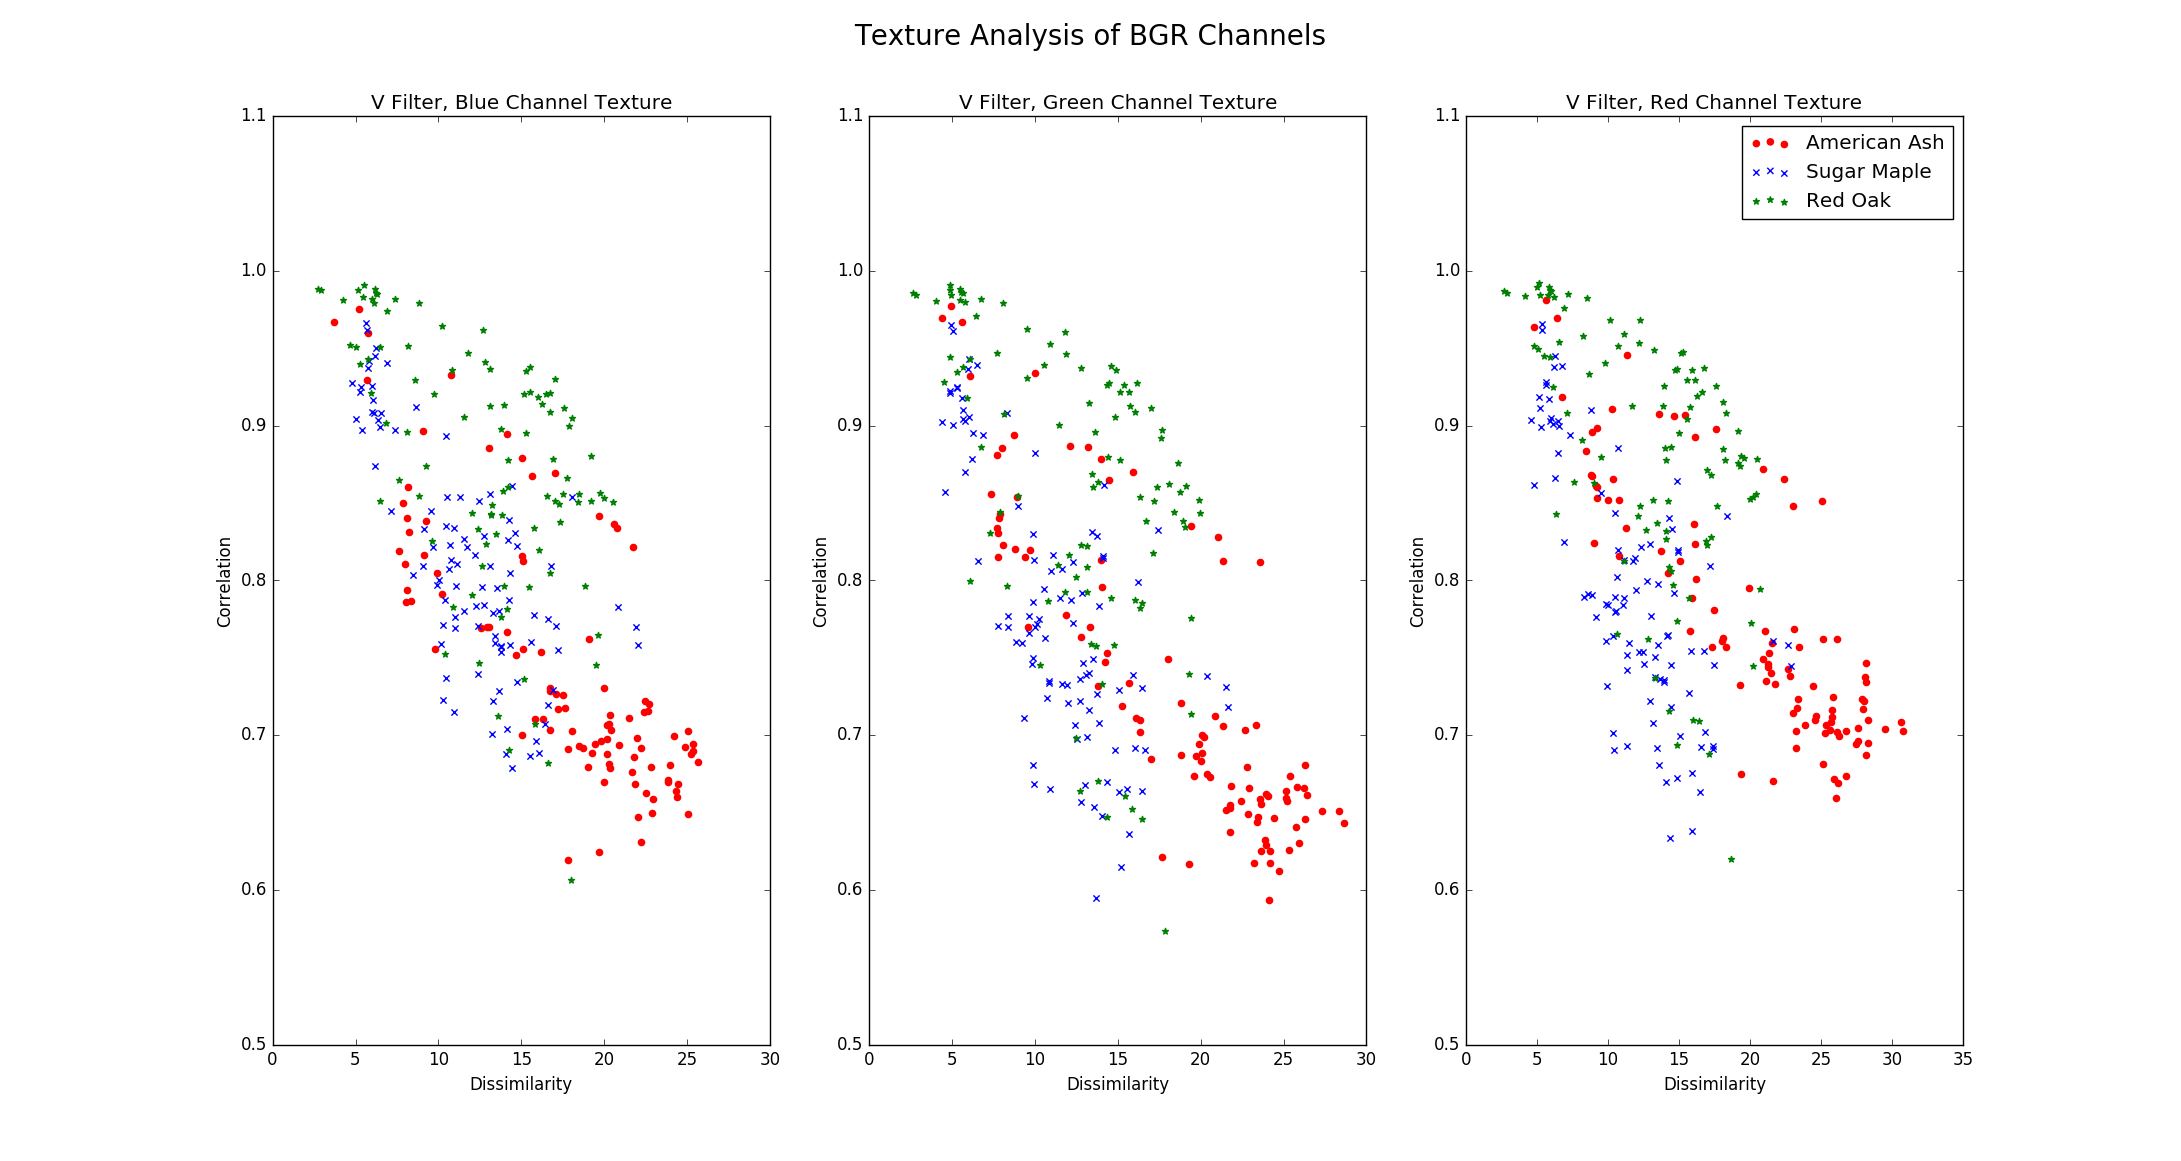
\includegraphics[scale=0.5]{/Sources/Appendix/GLCM-all-specles-V-specular.png}}
      \end{center}
      \caption{V filter GLCM Specular - All Species}
      \label{fig:polarization}
  \end{sidewaysfigure}
  \begin{sidewaysfigure}
      \begin{center}
          \makebox[\textwidth]{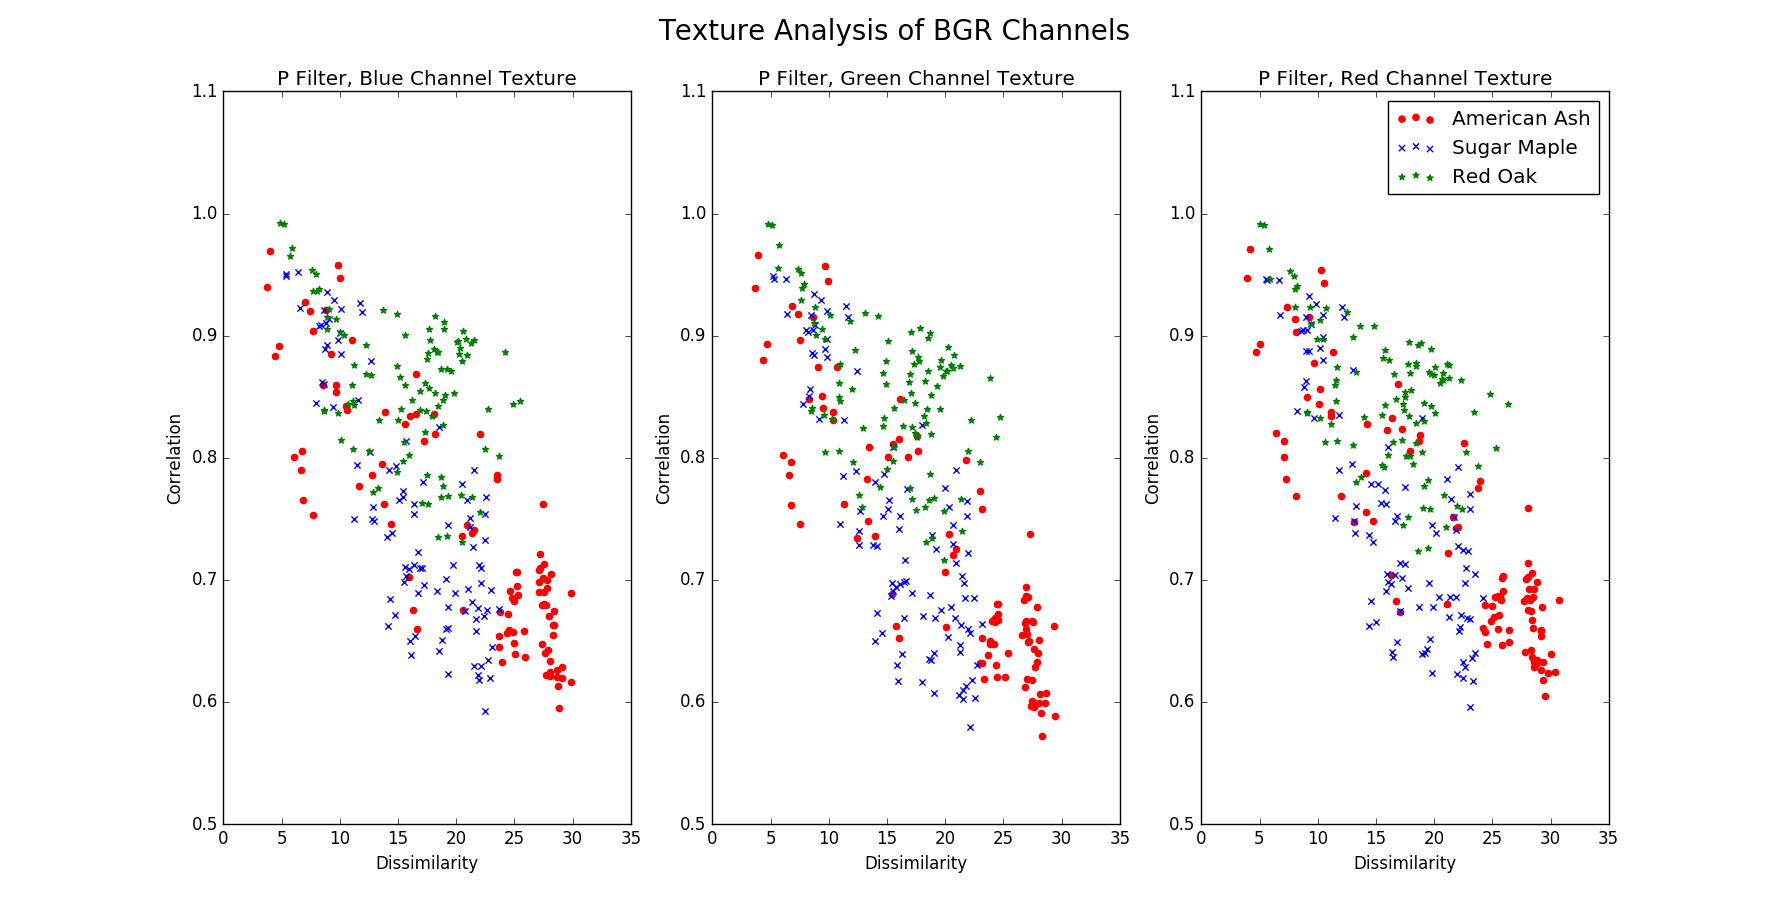
\includegraphics[scale=0.5]{/Sources/Appendix/GLCM-all-specles-P-specular.png}}
      \end{center}
      \caption{P filter GLCM Specular - All Species}
      \label{fig:polarization}
  \end{sidewaysfigure}
  \begin{sidewaysfigure}
      \begin{center}
          \makebox[\textwidth]{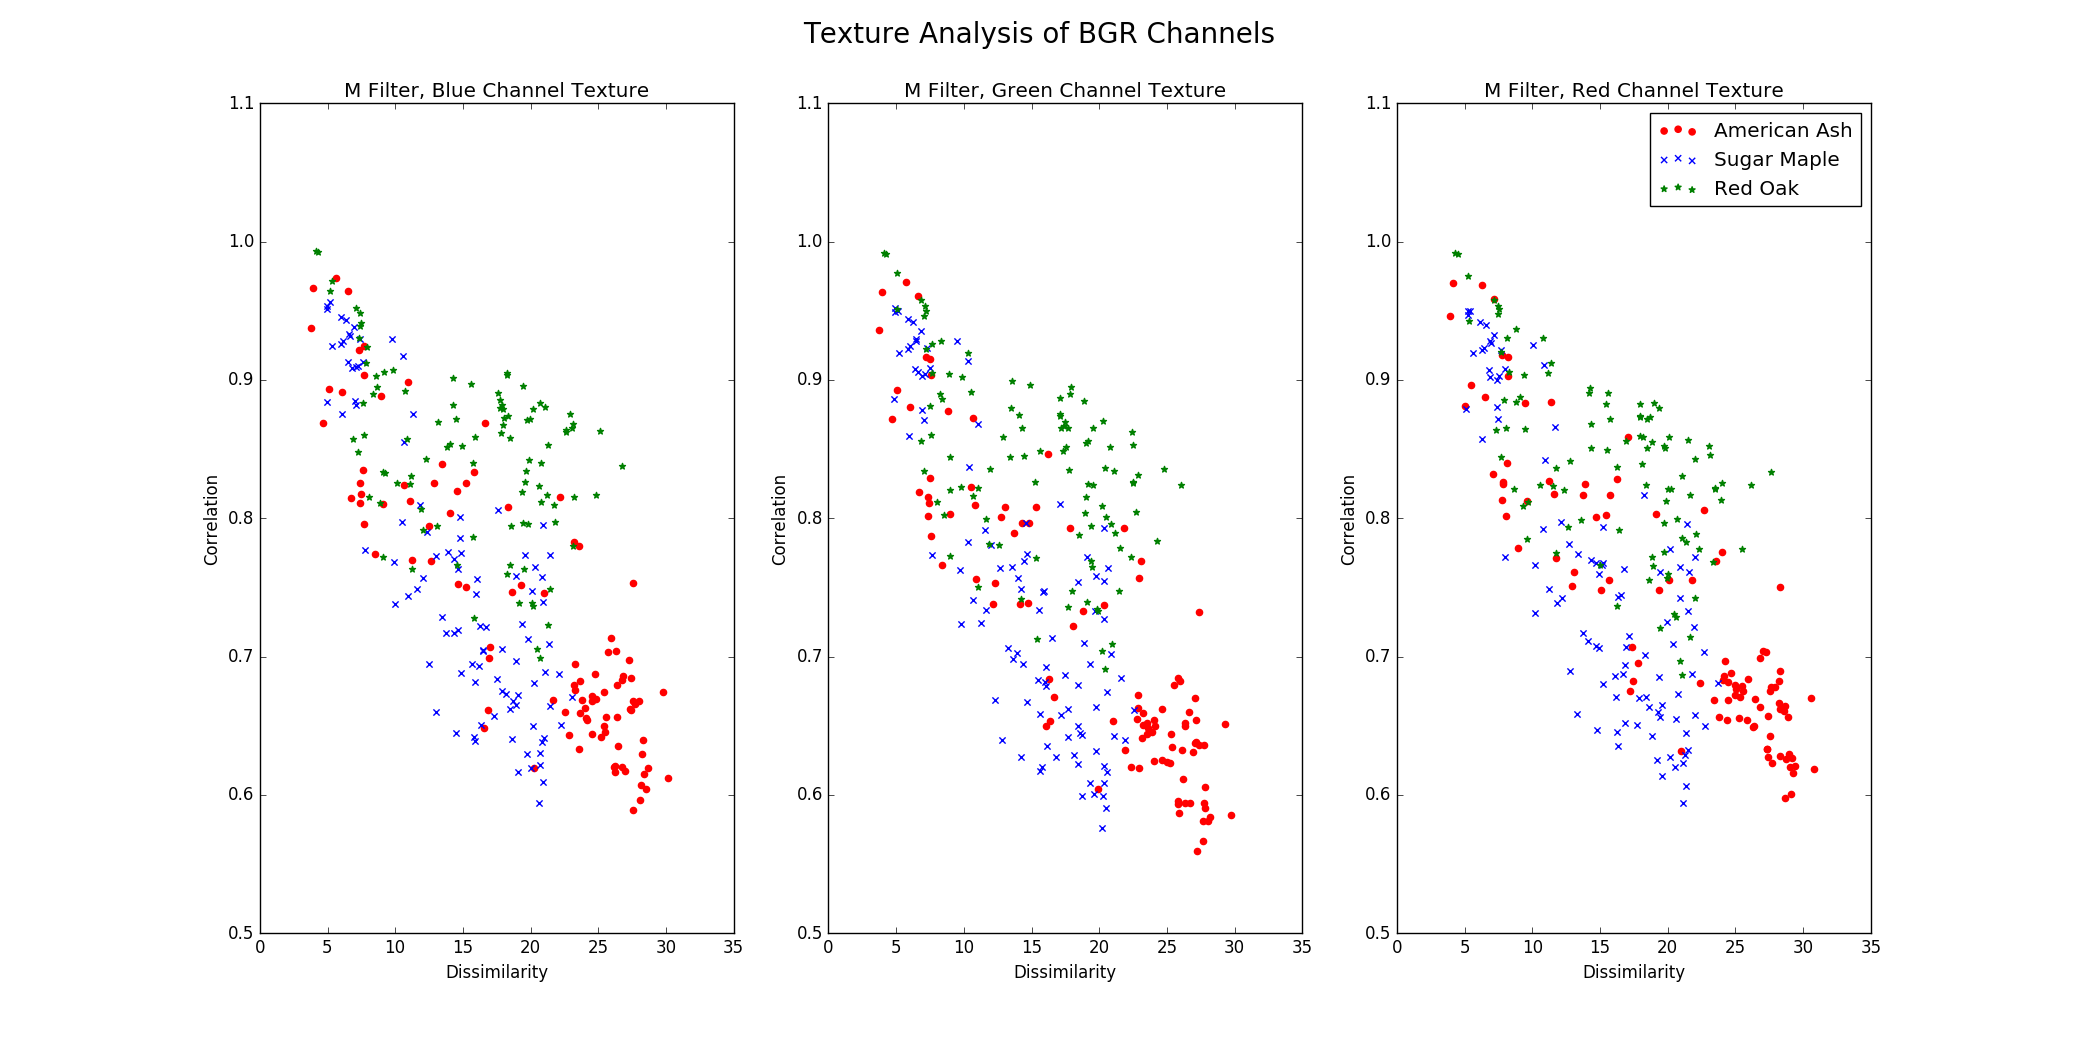
\includegraphics[scale=0.5]{/Sources/Appendix/GLCM-all-specles-M-specular.png}}
      \end{center}
      \caption{M filter GLCM Specular - All Species}
      \label{fig:polarization}
  \end{sidewaysfigure}
%%%%%%%%%%%%%%%%%%%%%%%%%%%%%%%%%%%%%%%%%%
%\subsection{Diffuse Results - All Species}
%%%%%%%%%%%%%%%%%%%%%%%%%%%%%%%%%%%%%%%%%%
  \begin{sidewaysfigure}
      \begin{center}
          \makebox[\textwidth]{\includegraphics[scale=0.5]{/Sources/Appendix/GLCM-H-all-species-diffuse-75.png}}
      \end{center}
      \caption{H filter GLCM Diffuse - All Species}
      \label{fig:polarization}
  \end{sidewaysfigure}
  \begin{sidewaysfigure}
      \begin{center}
          \makebox[\textwidth]{\includegraphics[scale=0.5]{/Sources/Appendix/GLCM-V-all-species-diffuse-75.png}}
      \end{center}
      \caption{V filter GLCM Diffuse - All Species}
      \label{fig:polarization}
  \end{sidewaysfigure}
  \begin{sidewaysfigure}
      \begin{center}
          \makebox[\textwidth]{\includegraphics[scale=0.5]{/Sources/Appendix/GLCM-P-all-species-diffuse-75.png}}
      \end{center}
      \caption{P filter GLCM Diffuse - All Species}
      \label{fig:polarization}
  \end{sidewaysfigure}
  \begin{sidewaysfigure}
      \begin{center}
          \makebox[\textwidth]{\includegraphics[scale=0.5]{/Sources/Appendix/GLCM-M-all-species-diffuse-75.png}}
      \end{center}
      \caption{M filter GLCM Diffuse - All Species}
      \label{fig:polarization}
  \end{sidewaysfigure}
%%%%%%%%%%%%%%%%%%%%%%%%%%%%%%%%%%%%%%%%%%%%%%
%\subsection{Specular Decomposition Results - Red Oak}
%%%%%%%%%%%%%%%%%%%%%%%%%%%%%%%%%%%%%%%%%%%%%%
\begin{sidewaysfigure}
    \begin{center}
        \makebox[\textwidth]{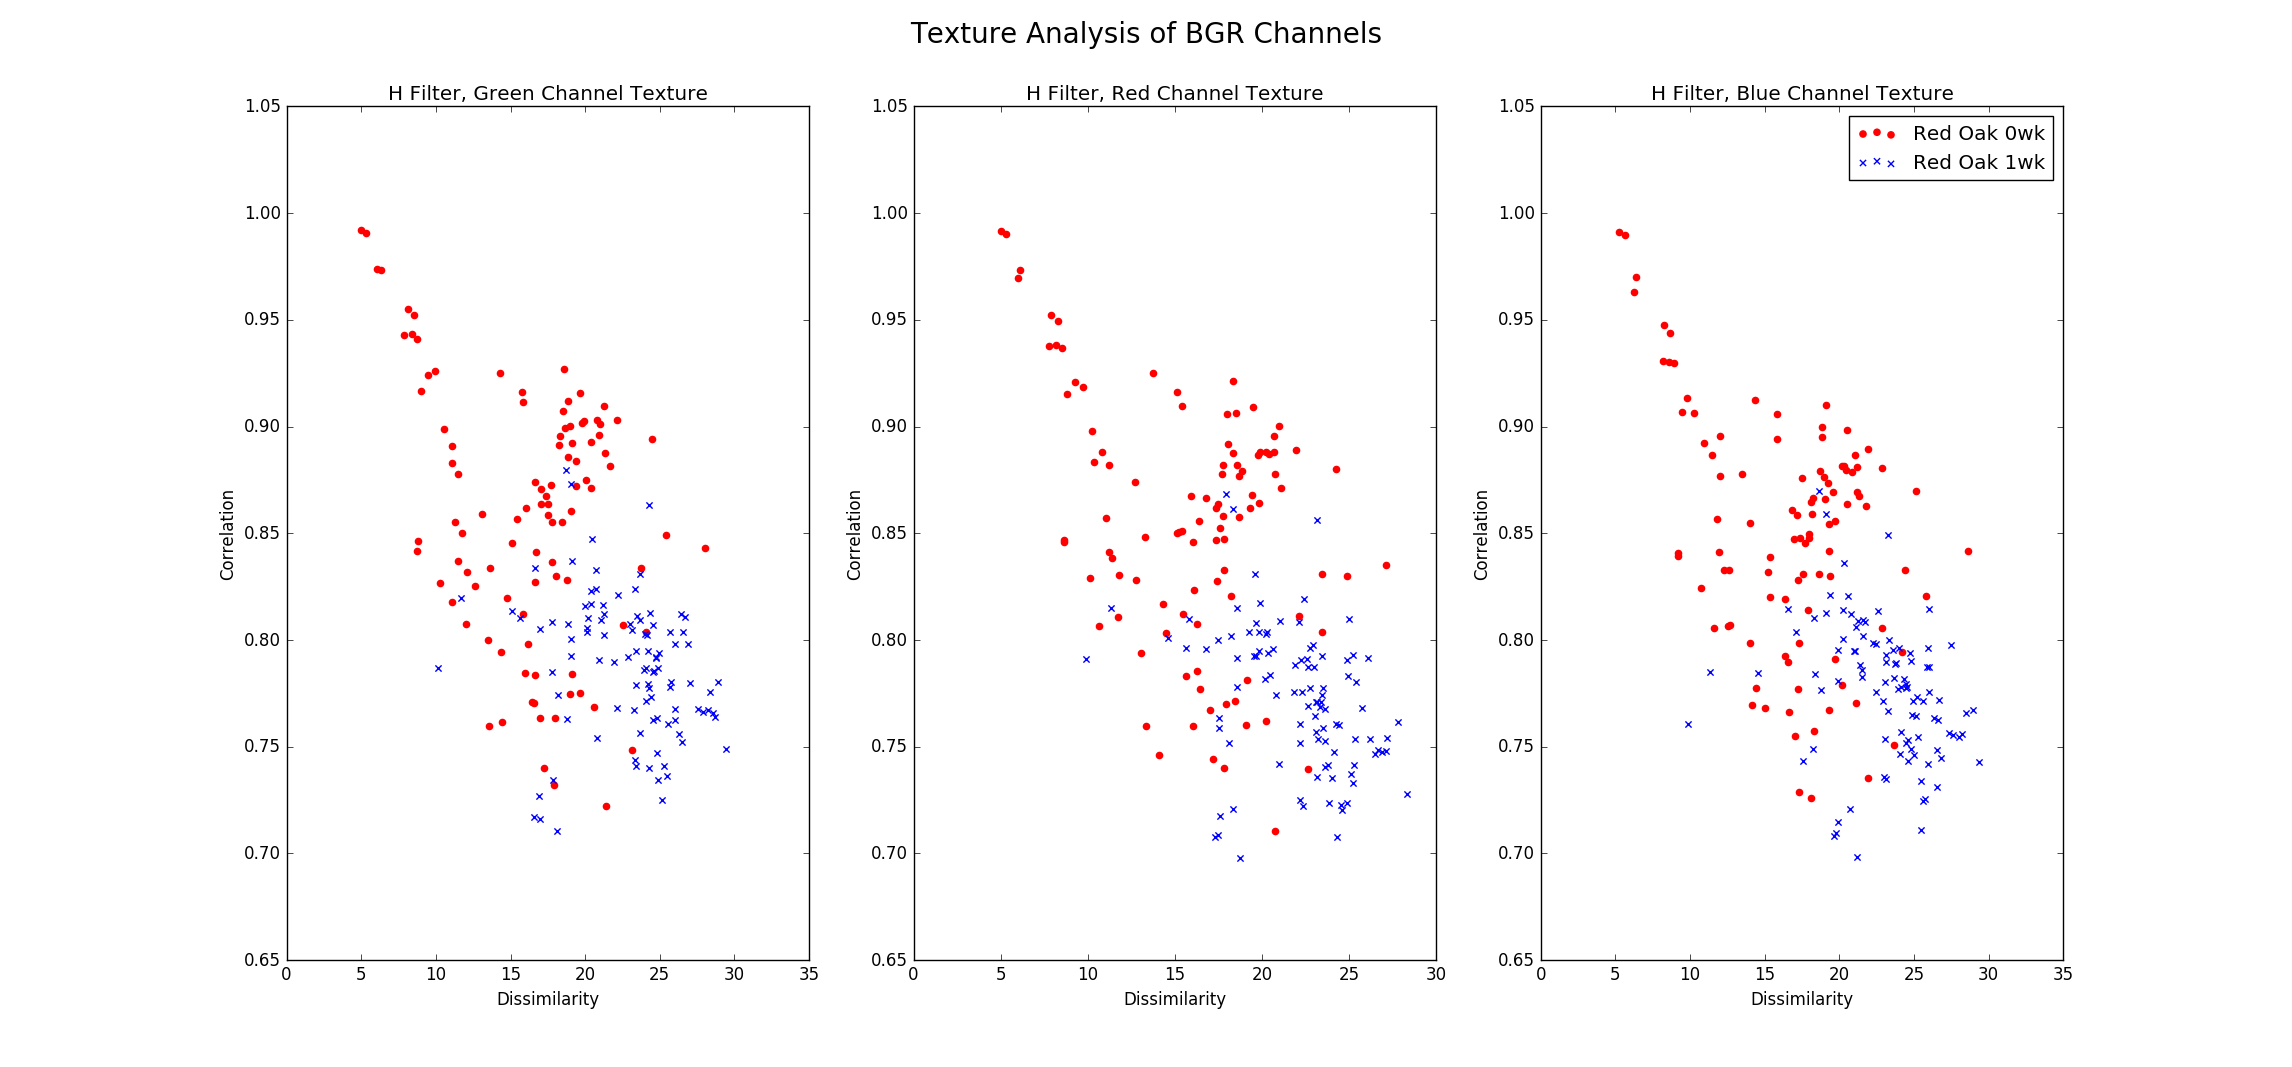
\includegraphics[scale=0.5]{/Sources/Appendix/GLCM-specular-oak-0wk-1wk-H.png}}
    \end{center}
    \caption{H filter GLCM Specular Decomposition - Red Oak}
    \label{fig:polarization}
\end{sidewaysfigure}
\begin{sidewaysfigure}
    \begin{center}
        \makebox[\textwidth]{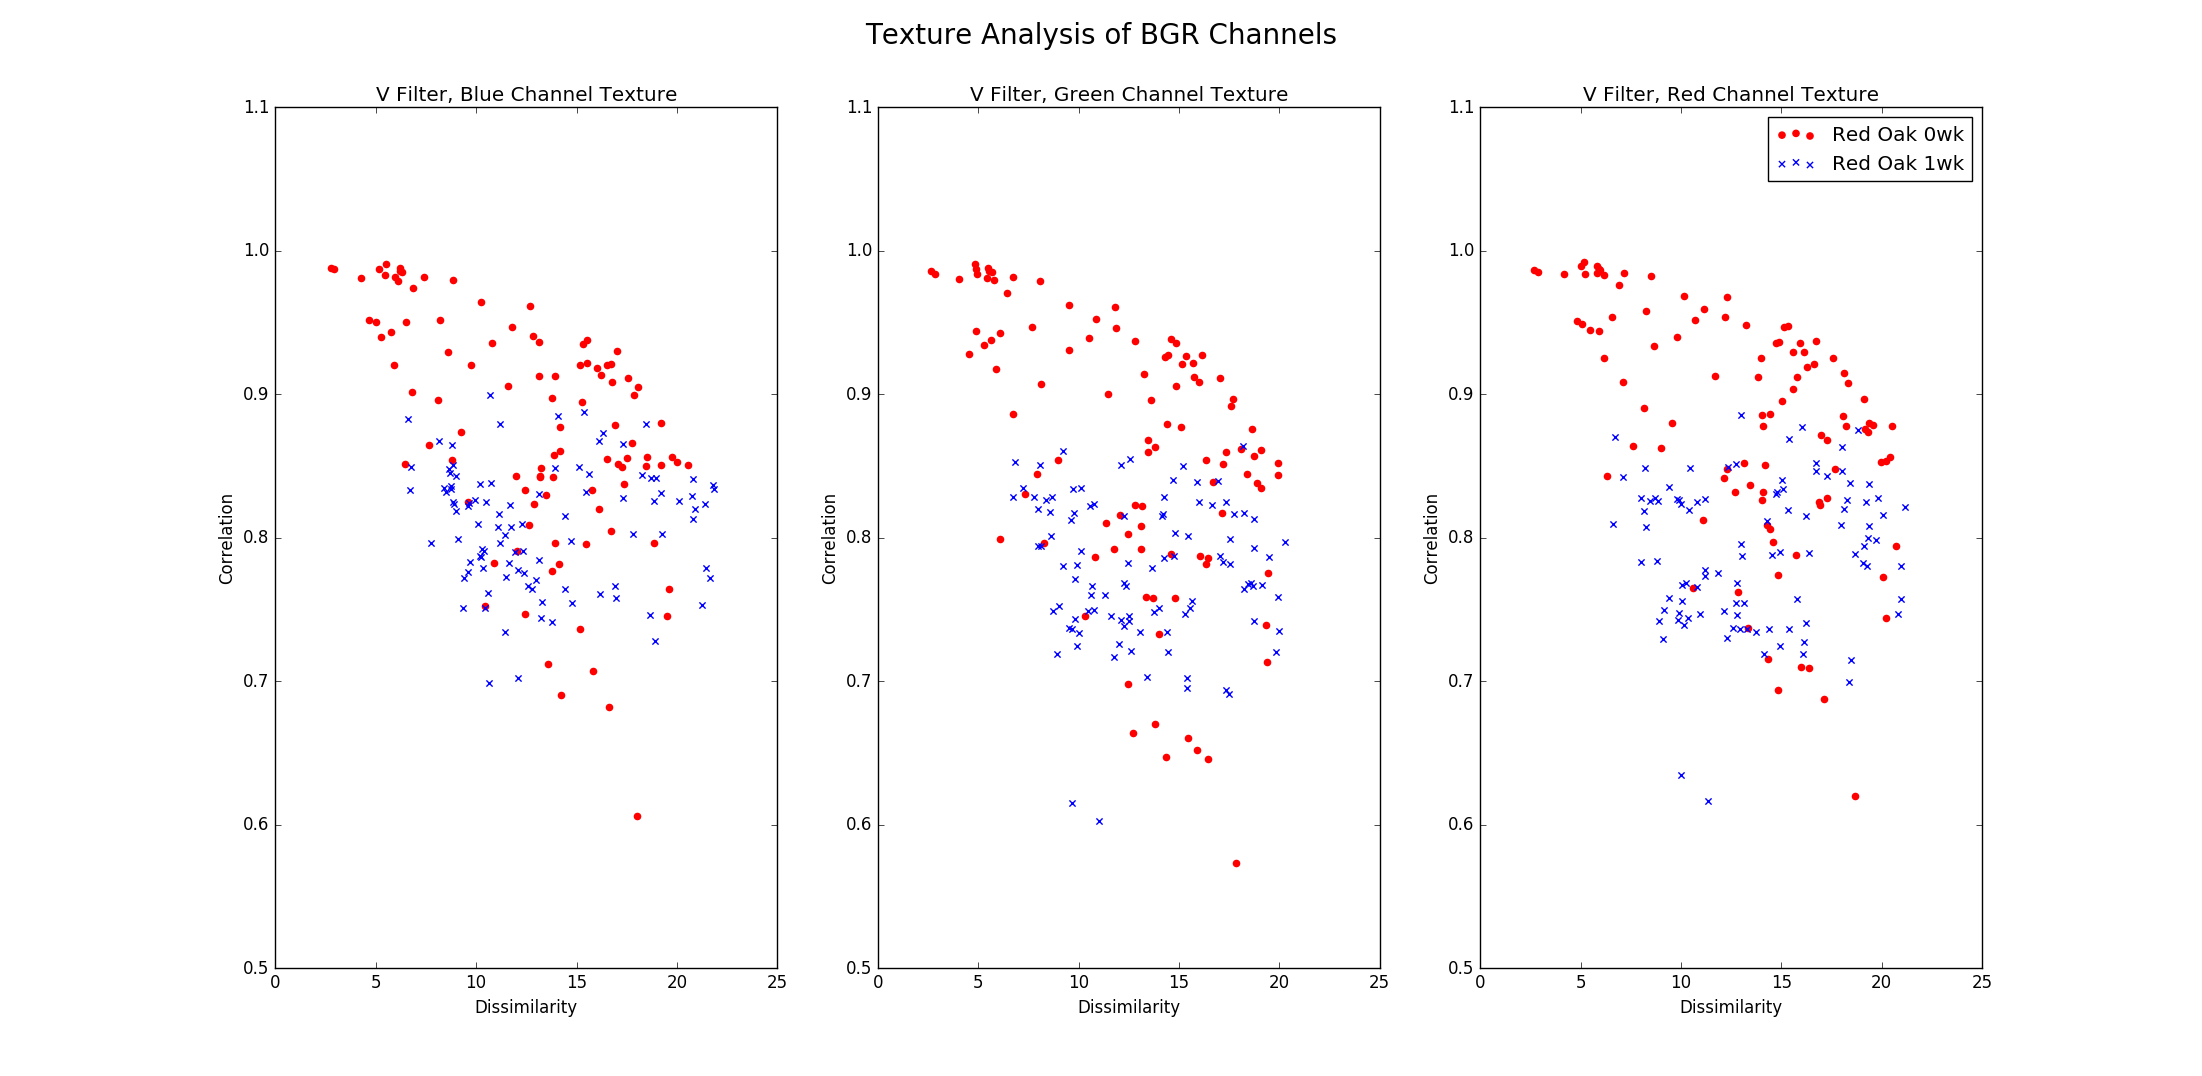
\includegraphics[scale=0.5]{/Sources/Appendix/GLCM-specular-oak-0wk-1wk-V.png}}
    \end{center}
    \caption{V filter GLCM Specular Decomposition - Red Oak}
    \label{fig:polarization}
\end{sidewaysfigure}
\begin{sidewaysfigure}
    \begin{center}
        \makebox[\textwidth]{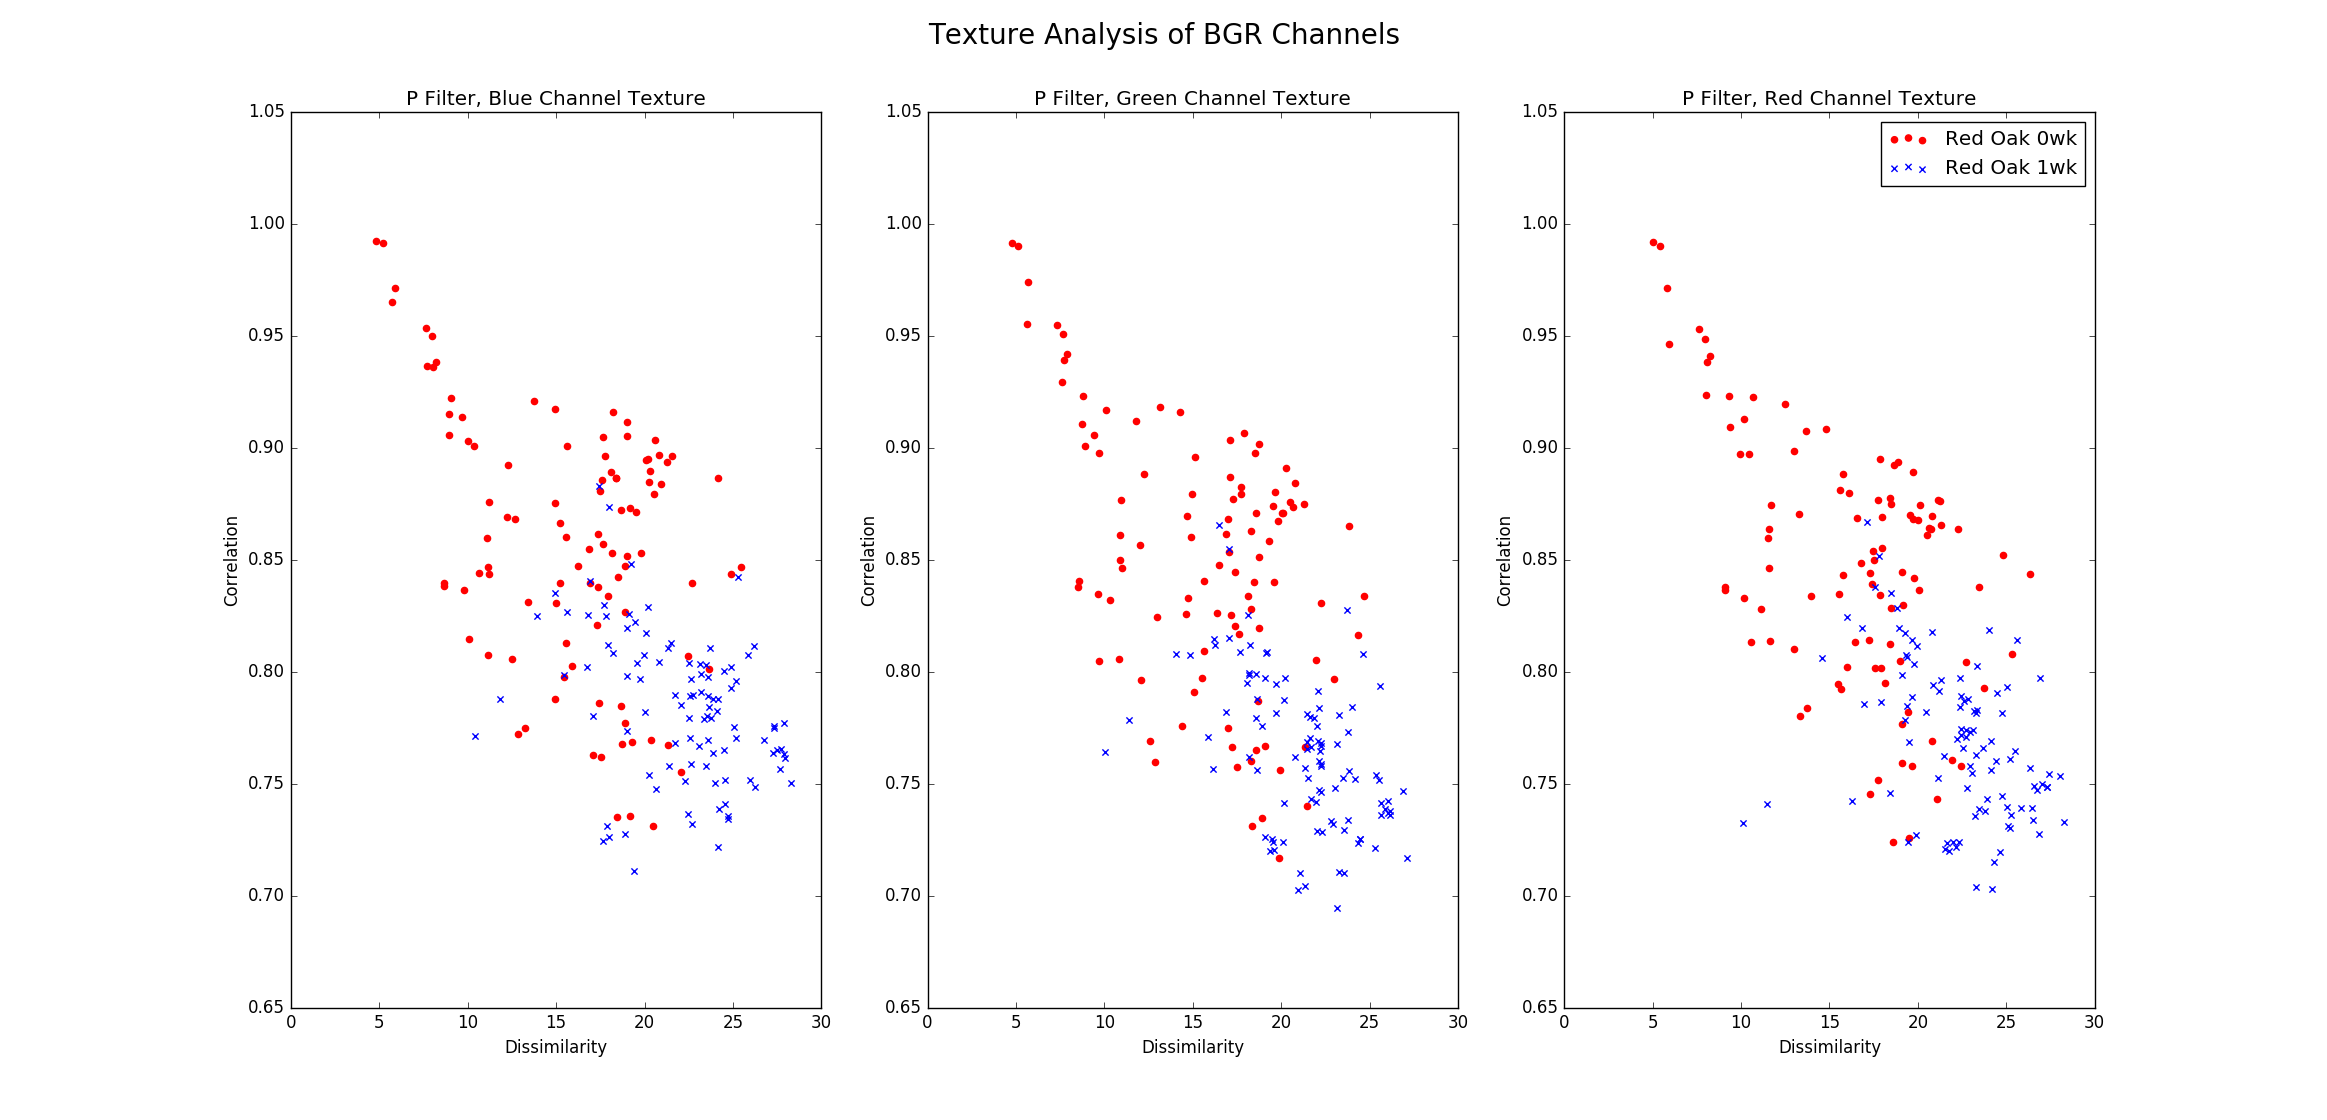
\includegraphics[scale=0.5]{/Sources/Appendix/GLCM-specular-oak-0wk-1wk-P.png}}
    \end{center}
    \caption{P filter GLCM Specular Decomposition - Red Oak}
    \label{fig:polarization}
\end{sidewaysfigure}
\begin{sidewaysfigure}
    \begin{center}
        \makebox[\textwidth]{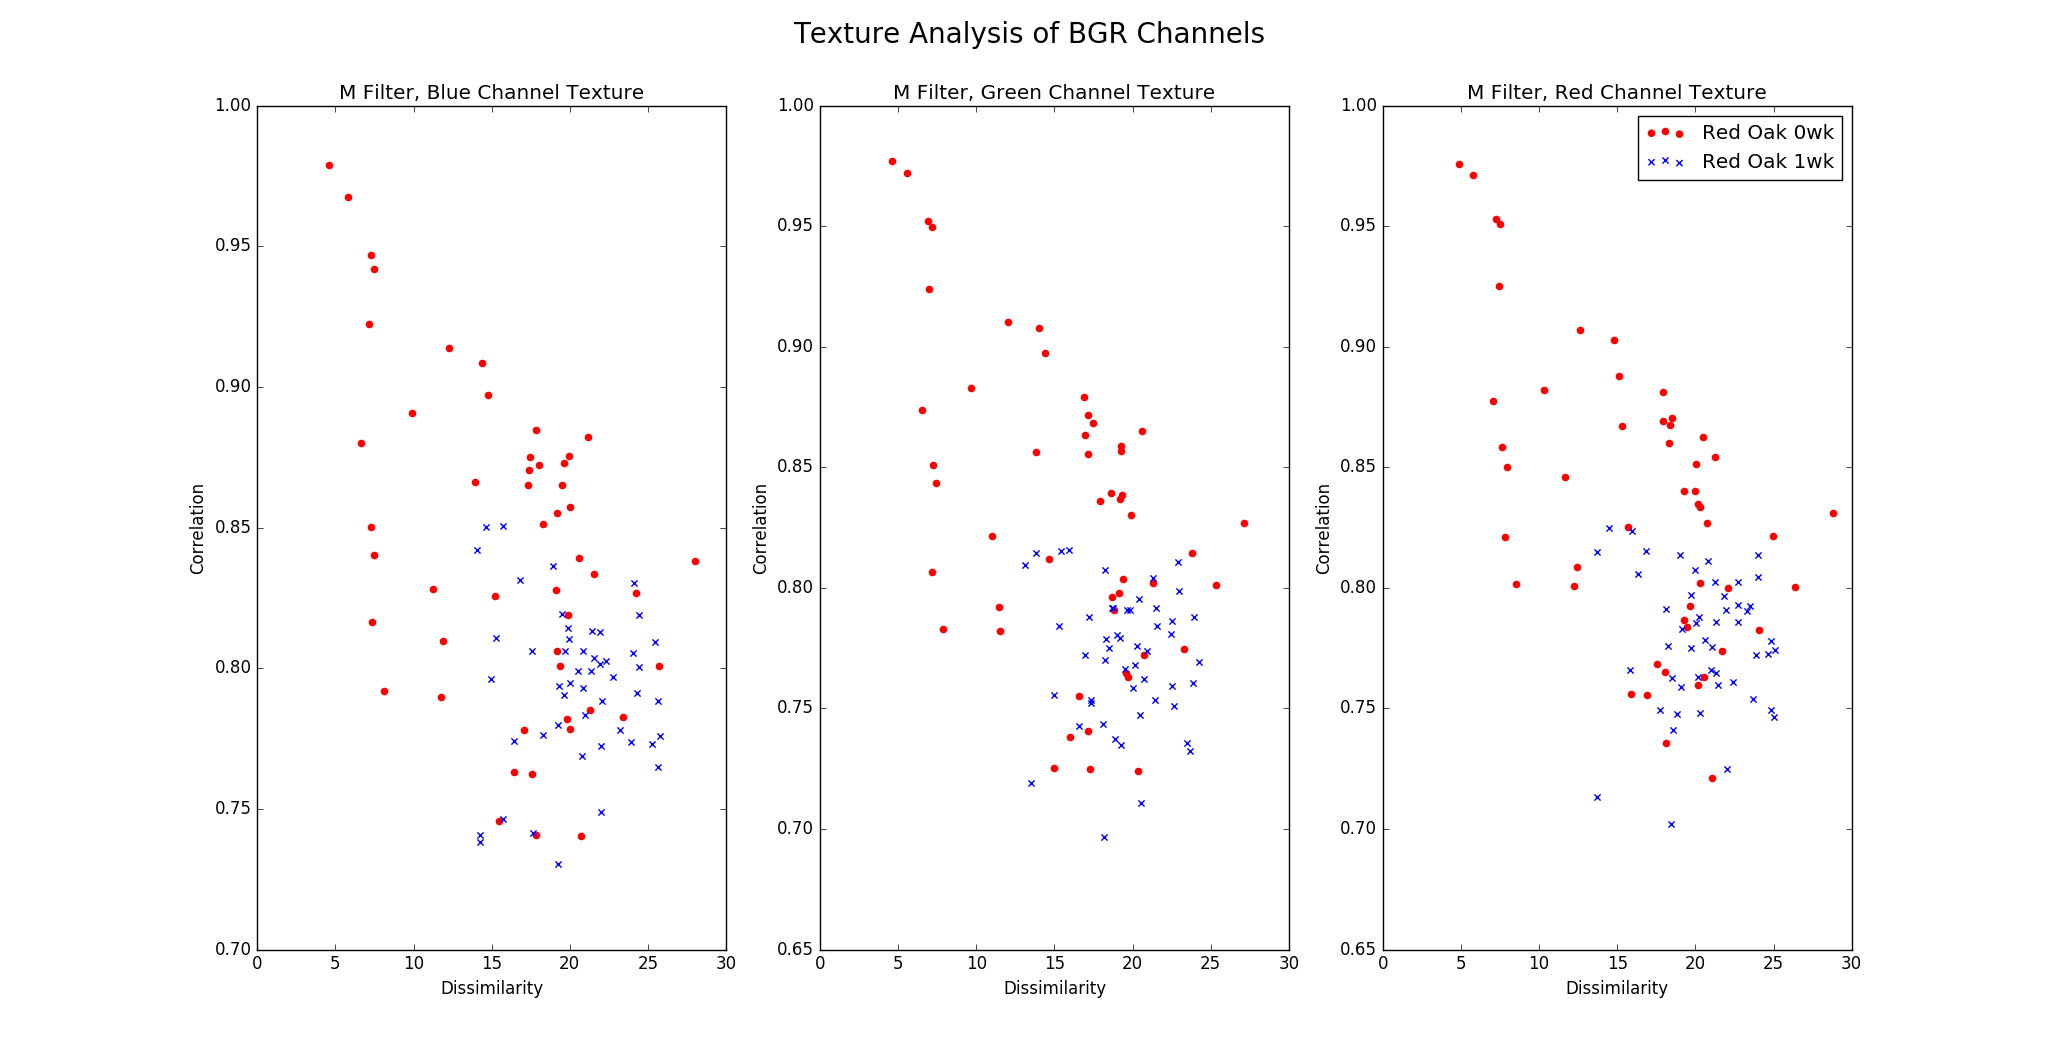
\includegraphics[scale=0.5]{/Sources/Appendix/GLCM-specular-oak-0wk-1wk-M.png}}
    \end{center}
    \caption{M filter GLCM Specular Decomposition - Red Oak}
    \label{fig:polarization}
\end{sidewaysfigure}
%%%%%%%%%%%%%%%%%%%%%%%%%%%%%%%%%%%%%%%%%%%%%%
%\subsection{Diffuse Decomposition Results - Red Oak}
%%%%%%%%%%%%%%%%%%%%%%%%%%%%%%%%%%%%%%%%%%%%%%
\begin{sidewaysfigure}
    \begin{center}
        \makebox[\textwidth]{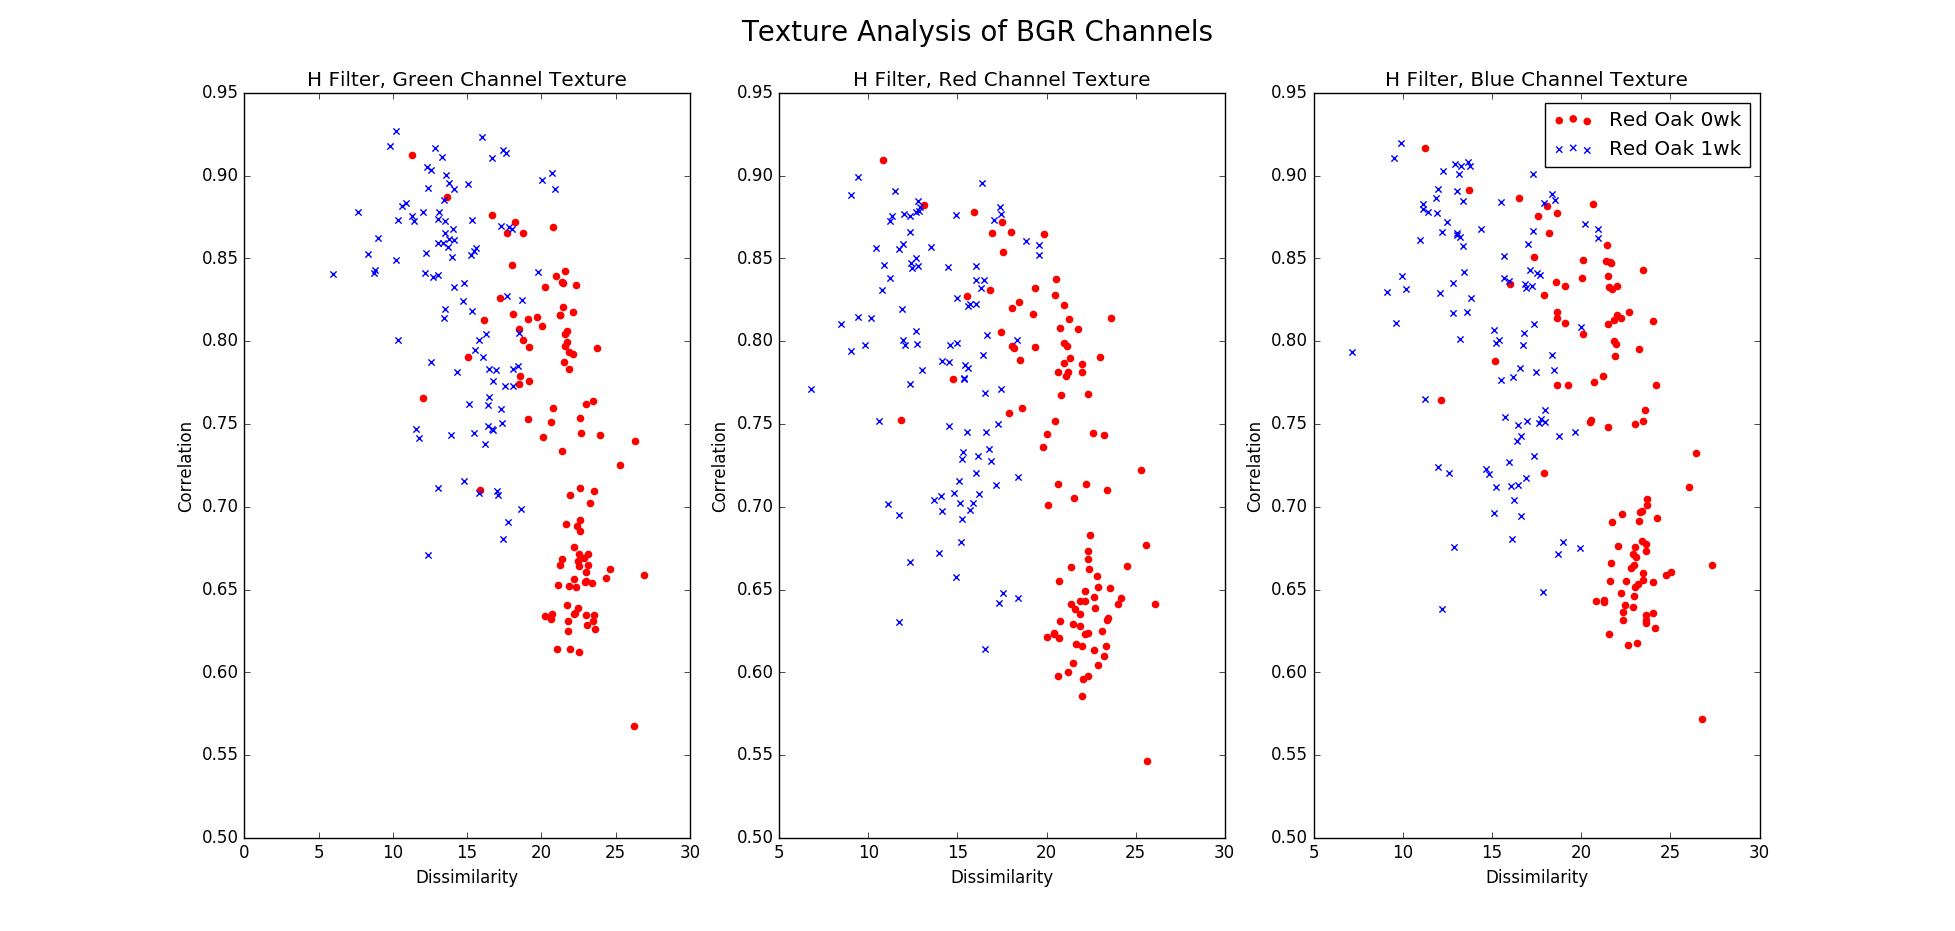
\includegraphics[scale=0.5]{/Sources/Appendix/GLCM-0wk-1wk-red-oak-H-diffuse.png}}
    \end{center}
    \caption{H filter GLCM Diffuse Decomposition - Red Oak}
    \label{fig:polarization}
\end{sidewaysfigure}
\begin{sidewaysfigure}
    \begin{center}
        \makebox[\textwidth]{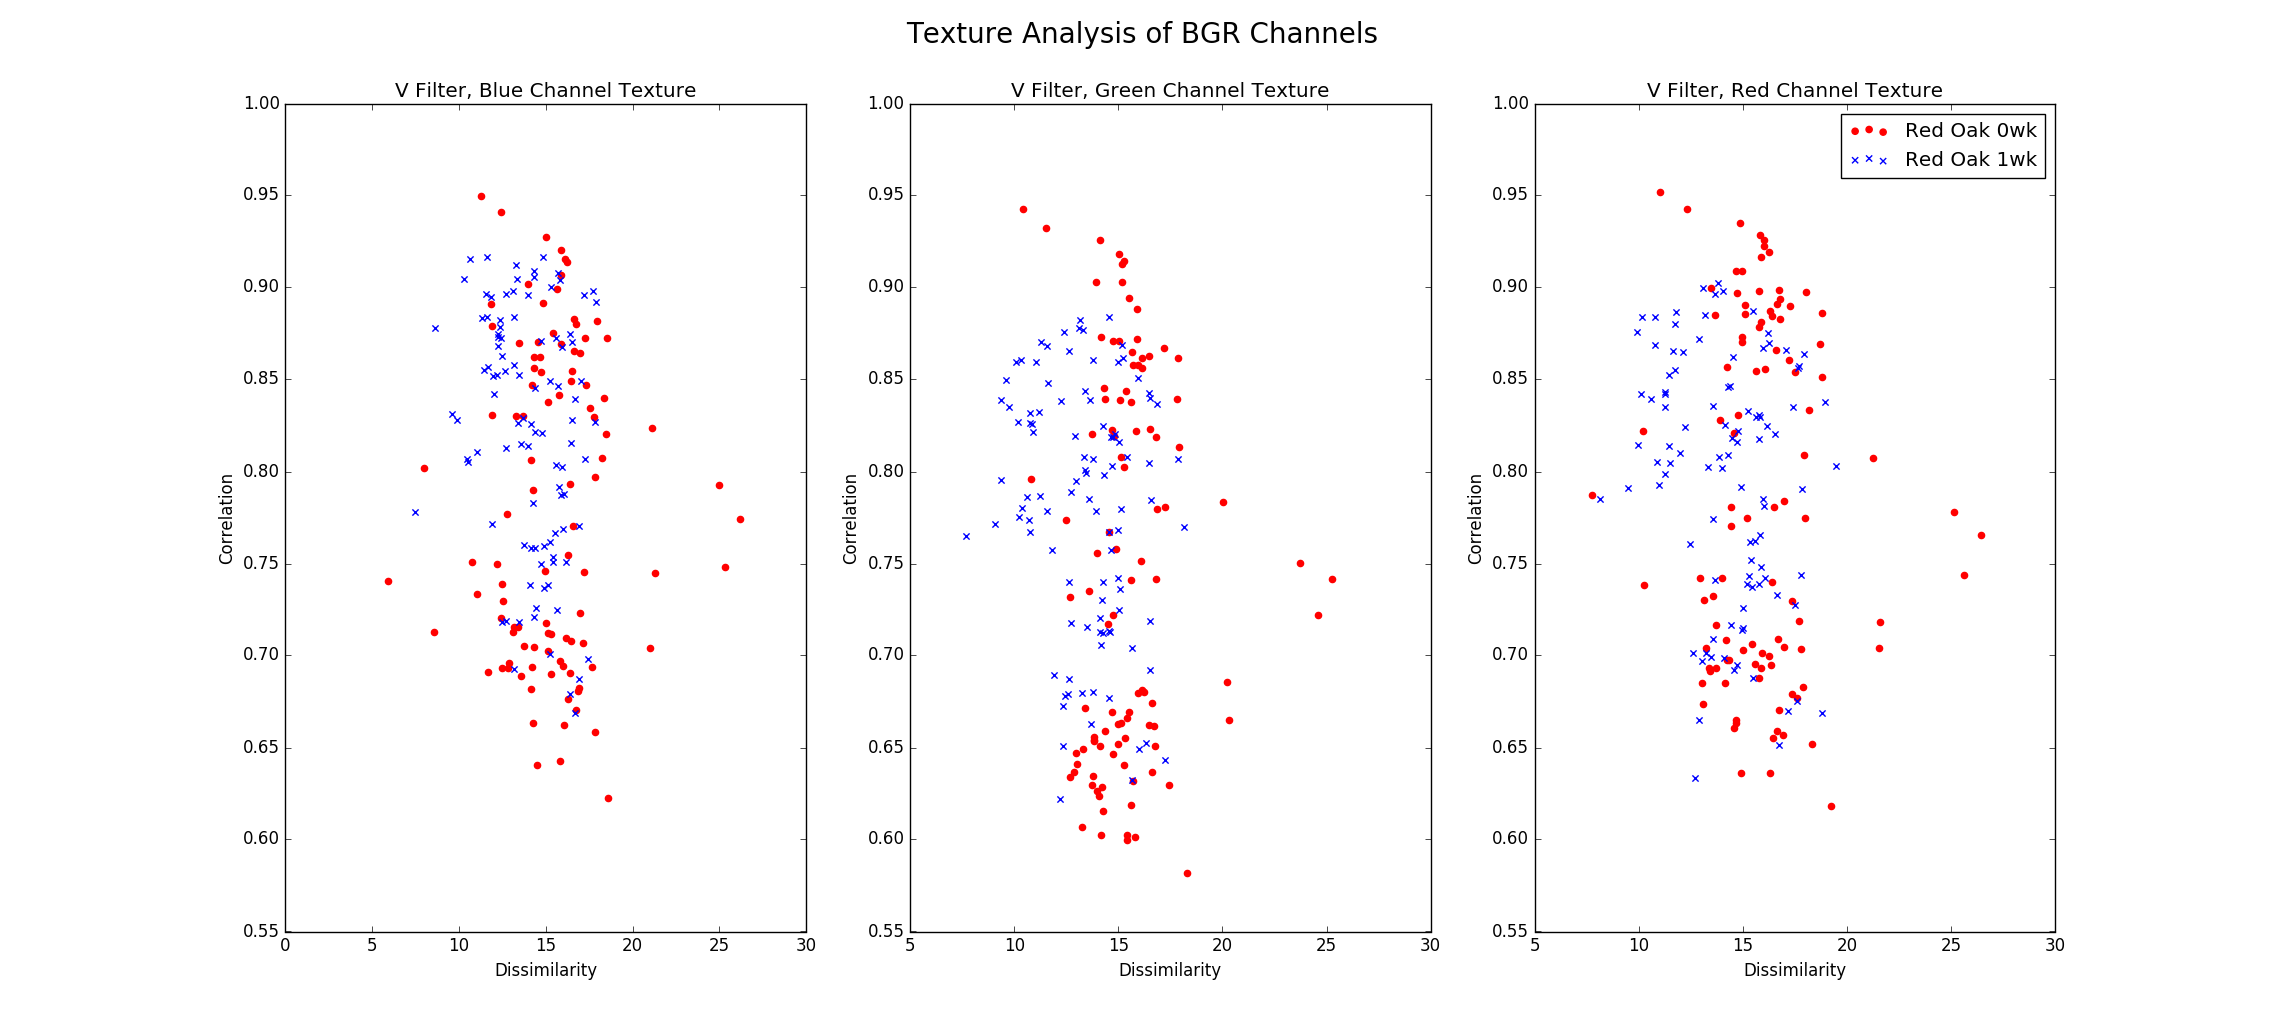
\includegraphics[scale=0.5]{/Sources/Appendix/GLCM-0wk-1wk-red-oak-V-diffuse.png}}
    \end{center}
    \caption{V filter GLCM Diffuse Decomposition - Red Oak}
    \label{fig:polarization}
\end{sidewaysfigure}
\begin{sidewaysfigure}
    \begin{center}
        \makebox[\textwidth]{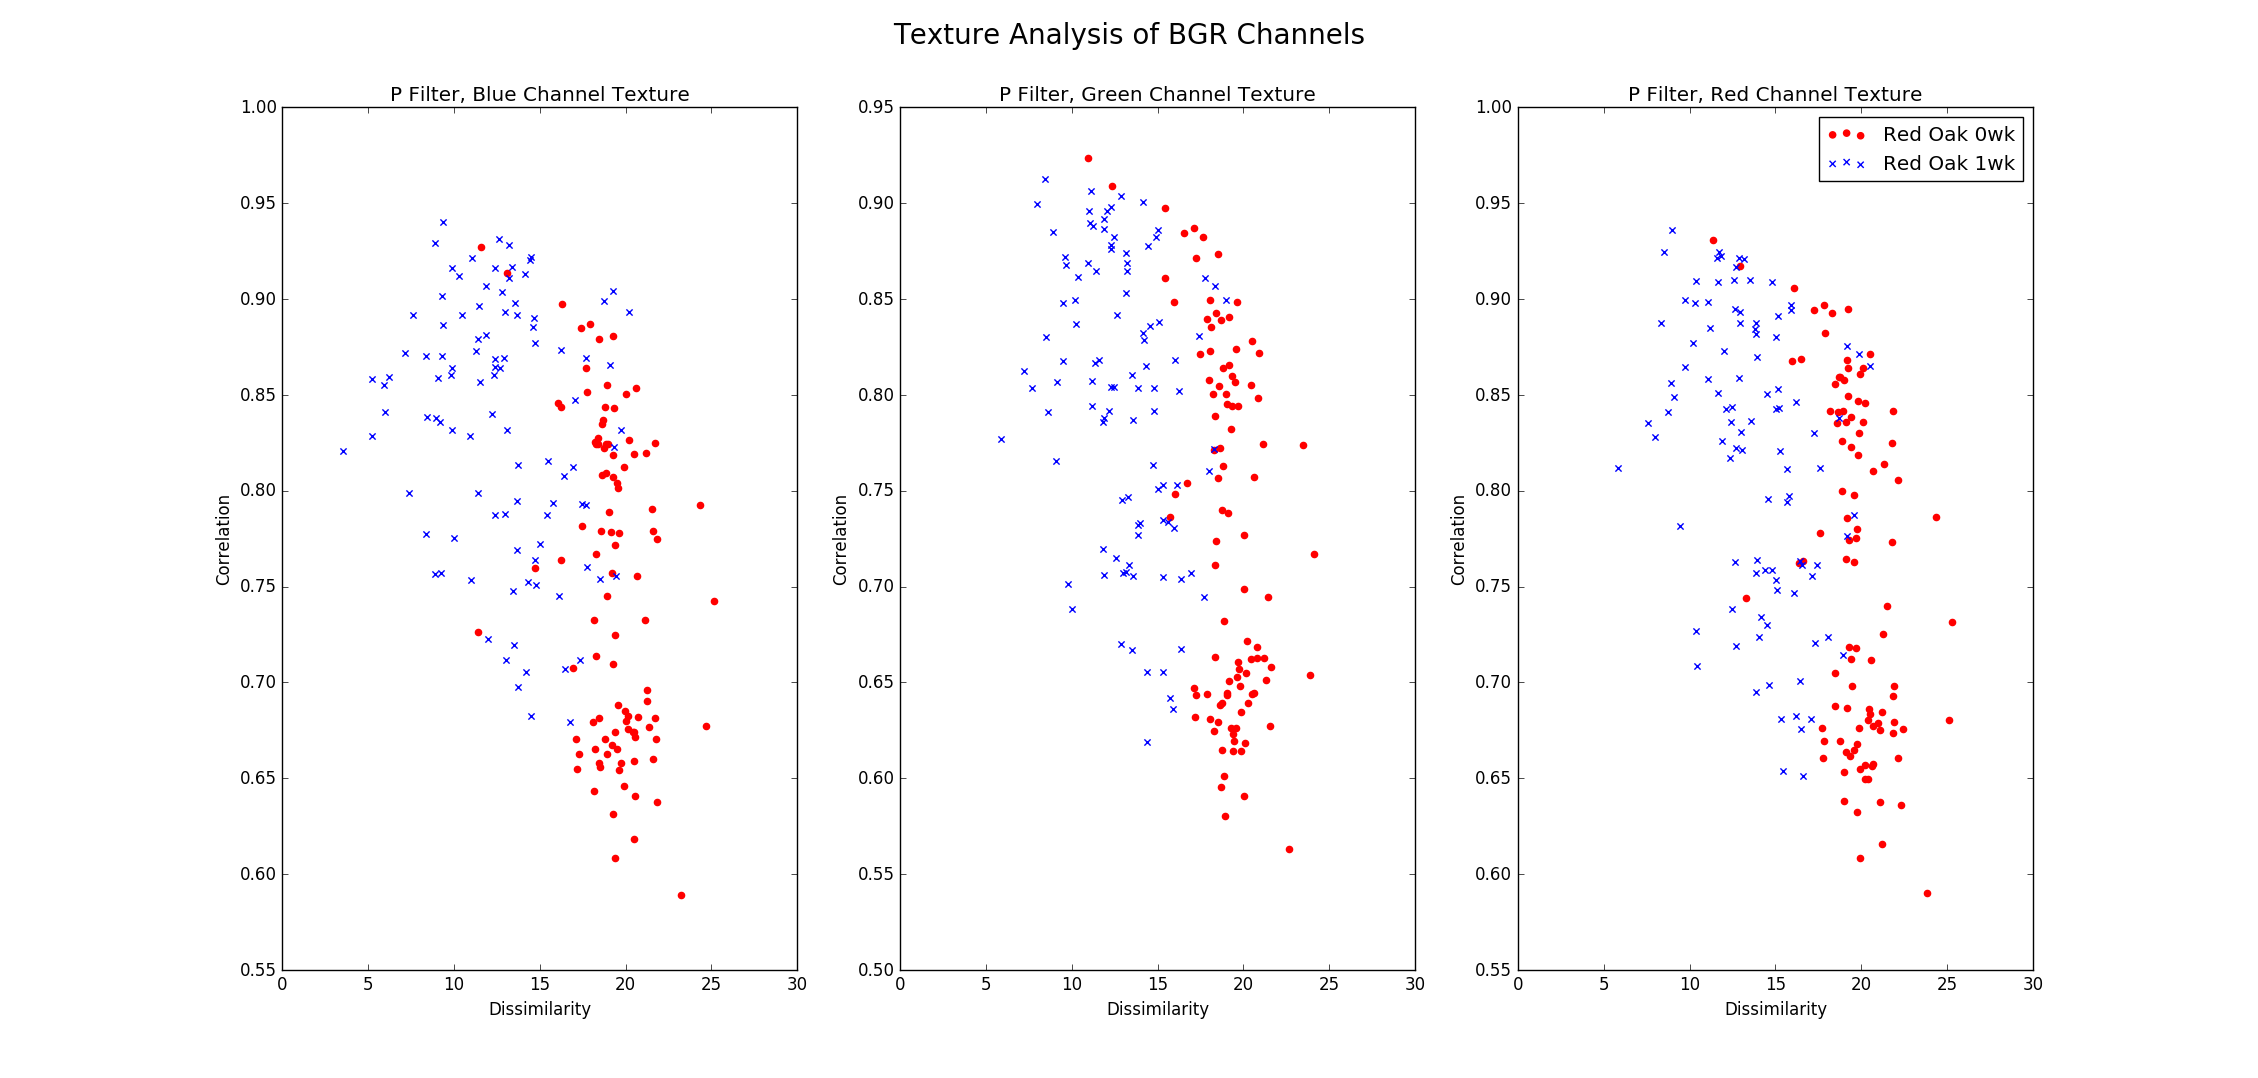
\includegraphics[scale=0.5]{/Sources/Appendix/GLCM-0wk-1wk-red-oak-P-diffuse.png}}
    \end{center}
    \caption{P filter GLCM Diffuse Decomposition - Red Oak}
    \label{fig:polarization}
\end{sidewaysfigure}
\begin{sidewaysfigure}
    \begin{center}
        \makebox[\textwidth]{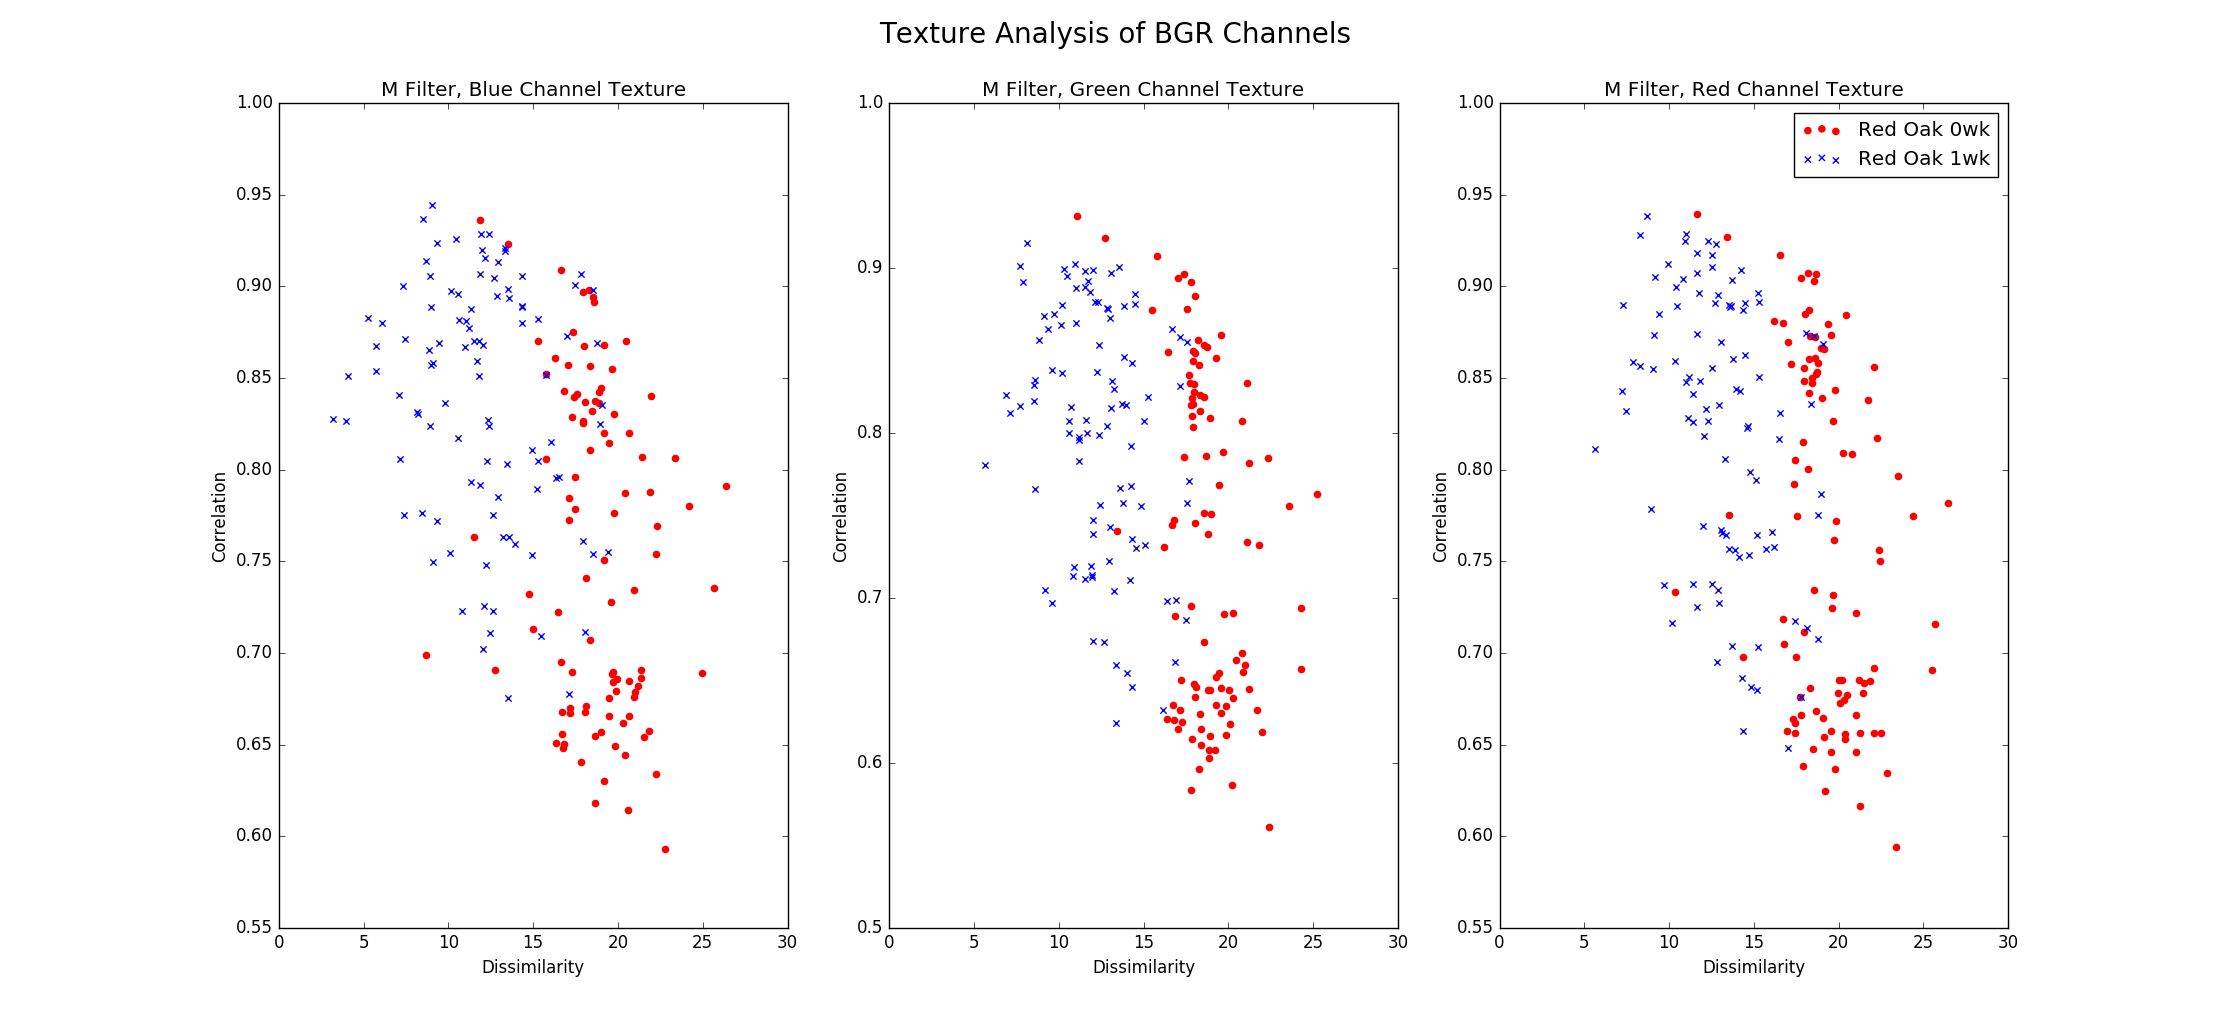
\includegraphics[scale=0.5]{/Sources/Appendix/GLCM-0wk-1wk-red-oak-M-diffuse.png}}
    \end{center}
    \caption{M filter GLCM Diffuse Decomposition - Red Oak}
    \label{fig:polarization}
\end{sidewaysfigure}
\end{appendices}
